\documentclass[11pt,a4paper]{article}

\usepackage[margin=1in]{geometry}
\usepackage{amsmath,amssymb}
\usepackage{booktabs}
\usepackage{graphicx}
\usepackage{hyperref}
\hypersetup{hypertexnames=false}
% Allow line breaks in \path and \url at / and _ (no xurl package required).
\makeatletter
\g@addto@macro\UrlBreaks{\do\/\do\_}
\makeatother
\usepackage{enumitem}
\usepackage{tabularx}
\usepackage{float}
\usepackage{xcolor}

% Visible ``marks'' for readers: gaps called out in the formal proposal review (April 2026).
\newcommand{\peerreviewmark}[1]{%
  \par\smallskip\noindent
  \fcolorbox{orange!65!black}{orange!6}{%
    \begin{minipage}{0.97\linewidth}
      \small\textbf{Improvement mark (proposal review).}\quad #1
    \end{minipage}}%
  \smallskip}

\title{Testing a spectral epidemic threshold for SIS on networks under heavy-tailed recovery}
\author{Jan Ruijgrok\\
  Open University of the Netherlands}
\date{April 2026}

\begin{document}
\maketitle

\begin{abstract}
Many infectious diseases do not confer lasting immunity, so infections may die out quickly or persist at low prevalence. Network SIS models often summarise ``control'' using compact rules that link spreading strength, mean infectious period, and connectivity---notably via the leading eigenvalue of the contact structure. Real recovery times can be irregular and heavy-tailed even when their average matches a simple reference case; our research asks whether such spectral mean-field thresholds still track outcomes in an explicit agent-based model. We implemented a group-recovery (grp) SIS formulation on a single fixed Erd\H{o}s--R\'enyi contact network, exported the contacts to obtain the spectral reference numerically, and ran replicated sweeps of infection strength under exponential, power-law, and lognormal recovery laws with the same mean recovery time, including trajectory output that compares microscopic prevalence to the homogeneous mean-field curve in the same implementation when extinction does not end runs early. Infection strengths at which half of stochastic replicates still carry the pathogen lie systematically above the mean-field prediction; differences between heavy-tailed and Markovian regimes in where that threshold falls are modest compared to this gap, whereas extinction timing depends more clearly on the recovery law. Overall, the spectral line is a useful conservative guide rather than a sharp critical value here, and heavy tails mainly reshape variability and transients more than they uniformly lower the survival threshold, partly qualifying the hypothesis that long tails alone strongly ease persistence at an unchanged average recovery duration.
\end{abstract}

\noindent\textbf{Keywords:} network epidemiology; SIS model; heavy-tailed recovery; agent-based simulation; spectral threshold; Erd\H{o}s--R\'enyi random graph.

\section*{Notation and symbols}
\phantomsection
\addcontentsline{toc}{section}{Notation and symbols}

\noindent
Table~\ref{tab:notation}: main mathematical symbols.\par
\noindent
Table~\ref{tab:netlogo-cols}: selected NetLogo/BehaviorSpace output names.

\begin{table}[H]
  \centering
  \small
  \caption{Mathematical notation (discrete-time SIS on an unweighted simple graph unless noted).}
  \label{tab:notation}
  \begin{tabularx}{\linewidth}{@{}l X@{}}
    \toprule
    \textbf{Symbol} & \textbf{Meaning} \\
    \midrule
    $N$ & Number of nodes (agents). \\
    $A$, $A_{ij}$ & Adjacency matrix; $A_{ij}{=}1$ if nodes $i,j$ are neighbours (unweighted graph). \\
    $\lambda_{\max}$ & Spectral radius (largest eigenvalue of $A$) for the exported contact network. \\
    $W$ & Random infectious period (recovery time) at the agent level; $\mathbb{E}[W]$ is its mean, fixed across recovery regimes in our comparisons. \\
    $\beta$ & Per-tick Bernoulli probability of transmission along an edge from an infected agent (NetLogo \emph{infection-prob}); one model tick is one discrete time step. \\
    $\tau$ & Effective transmission intensity; we use $\tau=\beta\,\mathbb{E}[W]$ (mean per-tick success probability times mean infectious duration in ticks). This matches the scale-free grouping used with continuous-time mean-field thresholds when $\mathbb{E}[W]$ is expressed in the same time units as $\beta$ (Section~\ref{sec:methods}). \\
    $\tau_c$ & Critical value of $\tau$ in spectral/mean-field theory; often $\tau_c\approx c/\lambda_{\max}$. \\
    $c$ & Dimensionless prefactor in threshold scaling (mean-field benchmark $c{=}1$). \\
    $\beta_{\mathrm{pred}}$ & Spectral prediction $\beta_{\mathrm{pred}}=1/(\lambda_{\max}\mathbb{E}[W])$ at $c{=}1$. \\
    $\tau_{\mathrm{pred}}$ & $\tau_{\mathrm{pred}}=\beta_{\mathrm{pred}}\mathbb{E}[W]=1/\lambda_{\max}$. \\
    $\hat{\beta}_{\mathrm{surv}\,50}$ & Smallest $\beta$ on the sweep grid for which at least $50\%$ of replicates are not extinct by the time limit (``survival'' threshold). \\
    $\hat{\tau}_{50}$ & $\hat{\beta}_{\mathrm{surv}\,50}\,\mathbb{E}[W]$. \\
    $\rho$ & Fraction infected (prevalence among $S{+}I$); microscopic vs.\ mean-field curves in experiment~\texttt{08}. \\
    $S$, $I$ & Susceptible and infected compartments (SIS). \\
    \bottomrule
  \end{tabularx}
\end{table}

\begin{table}[H]
  \centering
  \small
  \caption{NetLogo/BehaviorSpace metrics referenced in this report (names follow CSV export conventions).}
  \label{tab:netlogo-cols}
  \begin{tabularx}{\linewidth}{@{}l X@{}}
    \toprule
    \textbf{Name} & \textbf{Meaning} \\
    \midrule
    \texttt{bs-out-extinct} & Run ended in absorption with no infected agents ($1$) vs.\ infection still present at time limit ($0$). \\
    \texttt{bs-out-final-tick} & Tick at run termination. \\
    \texttt{bs-out-late-mean-prevalence} & Mean prevalence over a late time window (used in auxiliary persistence checks). \\
    \texttt{bs-out-prev-grp} / \texttt{bs-out-prev-mf} & Microscopic grp-SIS prevalence vs.\ homogeneous mean-field SIS prevalence (experiment~\texttt{08}). \\
    \bottomrule
  \end{tabularx}
\end{table}

\section{Introduction}

Many real-world infections do not give permanent immunity. People can be infected, recover, and then become infected again, sometimes multiple times in their life. Examples include common colds, certain sexually transmitted infections, and hospital-acquired infections. A central practical question is: \emph{when does an introduced infection die out quickly, and when can it keep circulating in a population for a long time?} This boundary between die-out and long-term persistence is often called the epidemic (or endemic) threshold.

In a basic SIS (susceptible--infected--susceptible) model on a network, each individual is either healthy and susceptible or currently infected, and recovery is typically assumed to follow a simple, memoryless process. A standard summary of how easily infection can take hold is an \emph{effective transmission} intensity $\tau$ that combines per-contact infection strength with the mean infectious period. Spectral arguments then predict an epidemic (endemic) threshold of the form
\[
  \tau_c \approx \frac{c}{\lambda_{\max}},
\]
where $\lambda_{\max}$ is the largest eigenvalue of the adjacency matrix and $c$ is a constant. In a homogeneous mean-field limit one often takes $c=1$; on a finite network, in discrete time, and with correlations beyond mean field, the effective $c$ need not be exactly one, but the scaling with $1/\lambda_{\max}$ remains the usual reference. Equivalently, at fixed mean recovery time $\mathbb{E}[W]$, the implied critical \emph{infection probability} is $\beta_c \approx \tau_c/\mathbb{E}[W] \approx c/(\lambda_{\max}\mathbb{E}[W])$. This spectral picture has been widely used and analysed in network epidemiology \cite{Chakrabarti2008,VanMieghem2011,PastorSatorras2015}.

However, real recovery times are often far from this idealised picture. Tang et al.\ introduce the grp-SIS framework as a generalisation of the basic SIS model, allowing more flexible recovery-time patterns for infected individuals, including heavy-tailed distributions, while keeping the same basic SIS structure of possible reinfection \cite{Tang2025}. Together with other work on SIS models with general or heavy-tailed recovery \cite{Cator2013}, this confirms that the \emph{shape} of the recovery-time distribution can strongly influence dynamics, even when the \emph{mean} recovery time is kept fixed.

What is much less clear from existing theory is whether the simple scaling $\tau_c \approx c/\lambda_{\max}$ (and the mean-field benchmark $c=1$) still describes the threshold well once we move away from exponential recovery towards more realistic, heavy-tailed recovery times. This question matters for practice because such rules of thumb are sometimes used to judge whether an infection is ``under control'' on a given contact structure. Agent-based modelling (ABM) offers a natural way to explore this gap: by simulating many individuals on an explicit contact network, with realistic recovery-time distributions, we can directly observe whether infections die out or persist under different parameter settings, without relying only on mean-field approximations (i.e., replacing detailed neighbour-to-neighbour correlations with average infection levels in the population).

In this project we therefore use a NetLogo agent-based SIS model on a simple random network (Erd\H{o}s--R\'enyi~\cite{ErdosRenyi1959} with about 2000 nodes and average degree around 6) as a numerical ``laboratory'' (see Figure~\ref{fig:er-network} for an example network). 


\begin{figure}[tbp]
  \centering
  
\includegraphics[width=0.6\textwidth]{er_network_example.png}
  \caption{Induced subgraph on a random subset of nodes from the exported ER edge list (seed $10001$), spring layout for visualisation only; full simulations use all $2000$ nodes. Highlighted nodes illustrate a possible infected set.}
  \label{fig:er-network}
\end{figure}

Within this setting we compare exponential (Markovian) recovery to heavy-tailed power-law and lognormal recovery, while keeping the mean recovery time $\mathbb{E}[W]$ fixed. This allows us to test how robust the spectral scaling $\tau_c \approx c/\lambda_{\max}$ remains in an explicit agent-based model and to see whether heavy-tailed recovery mainly shifts the epidemic threshold or primarily affects extinction times and variability.

\section{Methods}
\label{sec:methods}

\subsection*{Problem and research questions}

Our hypothesis is that heavy-tailed recovery makes it easier for the infection to persist in the population than a simple spectral threshold rule would suggest, even when the mean recovery time $\mathbb{E}[W]$ is held fixed. In other words, persistence may set in at a lower effective $\tau$ than the mean-field line $\tau_c \approx 1/\lambda_{\max}$ (i.e.\ $c=1$) would suggest, once recovery times are allowed to have long tails.

We address the following research questions to test this hypothesis in the agent-based model on Erd\H{o}s--R\'enyi networks with fixed parameters (about 2000 nodes and average degree around 6):

\begin{itemize}[leftmargin=*]
  \item \textbf{RQ1}. To what extent does the empirically observed threshold---in \emph{infection probability} or in $\tau$ (\emph{infection probability}$\times$\emph{mean recovery time})---agree with the spectral reference $\tau_c \approx c/\lambda_{\max}$ under the mean-field benchmark $c=1$, for an exponential (Markovian) recovery distribution?
  \item \textbf{RQ2}. How does the empirical threshold shift when the recovery distribution is replaced by Tang et al.'s power law or lognormal recovery, while keeping $\mathbb{E}[W]$ fixed?
  \item \textbf{RQ3}. On this Erd\H{o}s--R\'enyi topology (fixed \emph{number of nodes} and \emph{average degree}), does heavy-tailed recovery (power law or lognormal) lead to a systematically different empirical threshold (in terms of infection probability) compared to exponential recovery, or are differences mainly visible in extinction-time distributions and prevalence variability?
\end{itemize}

\subsection*{Research setup}

\begin{itemize}[leftmargin=*]
  \item \textbf{Simulated world}. Individuals are nodes on an Erd\H{o}s--R\'enyi graph~\cite{ErdosRenyi1959} generated in NetLogo with about \emph{number of nodes}${}=2000$ and \emph{average degree}${}=6$. The ER baseline uses a fixed \texttt{expt-seed} (aligned with the exported edge list for $\lambda_{\max}$) so that exponential, power-law, and lognormal recovery are compared on the \emph{same} network instance; BehaviorSpace \texttt{repetitions} supply process noise. That choice prioritises internal validity over graph-ensemble variation; an \emph{Improvement mark} under Methods flags extending the design to several independent ER draws.

  \item \textbf{Infection process}. A standard agent-based SIS process runs on each such network: infection can spread along links; after recovery an individual can be infected again. The NetLogo model sets \emph{infection probability} (strength of transmission per time step along a link).

  \item \textbf{What we vary}. (i)~The infection strength \emph{infection probability}, swept over many values. (ii)~The recovery time pattern: first a simple ``memoryless'' exponential pattern, then two heavy-tailed options implemented as in Tang et al.\ (power law and lognormal).

  \item \textbf{What we keep fixed}. The graph, the generative specification (ER, \emph{number of nodes}, \emph{average degree}), and the \emph{mean recovery time}, so comparisons between recovery regimes are fair at the same $\mathbb{E}[W]$.

  \item \textbf{Reference prediction from the network}. The contact list is exported to a CSV file. In Python, we compute the largest eigenvalue $\lambda_{\max}$ of the adjacency matrix. The mean-field spectral reference is $\tau_c \approx 1/\lambda_{\max}$ (i.e.\ $c=1$ in $\tau_c \approx c/\lambda_{\max}$). At fixed mean recovery time $\mathbb{E}[W]$, the corresponding critical \emph{infection probability} is $\beta_{\mathrm{pred}} = 1/(\lambda_{\max}\,\mathbb{E}[W])$, which marks the spectral prediction on the $\beta$ axis.
\end{itemize}

\subsection*{Measurement, empirical threshold rule, and estimation protocol}

\begin{itemize}[leftmargin=*]
  \item \textbf{Run outcome}. Each BehaviorSpace run ends when an infection-free absorbing state is reached or when simulated time reaches a configured cap (\texttt{max-ticks}, here $10{,}000$ for experiments \texttt{05}--\texttt{07}). We record whether the run is classified extinct (\texttt{bs-out-extinct}${}=1$), the final tick, and late-window mean prevalence (\texttt{bs-out-late-mean-prevalence}) for auxiliary persistence checks. Simulations use NetLogo~7.0.3 (BehaviorSpace table exports in \path{output/raw/}).

  \item \textbf{Persistence vs.\ extinction at the horizon}. A replicate counts as \emph{surviving} (still persistent) if \texttt{bs-out-extinct}${}=0$, i.e.\ at least one infected agent remains at the time limit; otherwise it is \emph{extinct}. This is the operational rule behind ``typically persists'' in the proposal: it is \emph{not} a quasi-stationary distribution estimate, but a finite-horizon survival indicator.

  \item \textbf{Design size and sweep schedule}. For each recovery regime, experiments \texttt{05}--\texttt{07} use \texttt{repetitions}${}=24$ per $(\beta,\text{regime})$ and a uniform stepped sweep of \texttt{infection-prob} from $0.018$ to $0.048$ in steps of $0.002$ ($16$ values), i.e.\ $384$ stochastic runs per regime unless runs fail validation. The same schedule is applied in all three recovery laws so that differences are not confounded by replication count.

  \item \textbf{Grid-based $50\%$ survival threshold $\hat{\beta}_{\mathrm{surv}\,50}$}. For each $\beta$ on the grid, the \emph{survival rate} is the fraction of replicates with \texttt{bs-out-extinct}${}<0.5$. We define $\hat{\beta}_{\mathrm{surv}\,50}$ as the \emph{smallest} $\beta$ on the grid at which this fraction is at least $50\%$, implemented in \path{scripts/threshold_estimators.py}. If the curve never reaches $50\%$ below the largest $\beta$, the estimator equals the largest grid point (right-censoring). Stratified bootstrap confidence intervals ($n{=}400$ resamples over the $\beta$ grid, stratifying by $\beta$) use the same rule.

  \item \textbf{Uncertainty reporting}. Bootstrap intervals reflect stochastic replicate noise conditional on the fixed network; they do not add a second layer of graph-realisation uncertainty because a single ER instance is used for the main comparison.

  \item \textbf{Effective transmission}. We report $\hat{\tau}_{50}=\hat{\beta}_{\mathrm{surv}\,50}\,\mathbb{E}[W]$ and compare $\hat{\tau}_{50}/\tau_{\mathrm{pred}}$ to the mean-field benchmark $c{=}1$.

  \item \textbf{Link to RQ1--RQ3}. \textbf{RQ1}: agreement between $\hat{\beta}_{\mathrm{surv}\,50}$ and $\beta_{\mathrm{pred}}$ under exponential recovery. \textbf{RQ2}: shifts under power-law and lognormal recovery at fixed $\mathbb{E}[W]$. \textbf{RQ3}: extinction-time and variability differences even when $\hat{\beta}_{\mathrm{surv}\,50}$ is similar.
\end{itemize}

\paragraph{Discrete-time infection probability and continuous-time $\tau$.}
In the NetLogo implementation, one \emph{tick} is one discrete time step; \emph{infection-prob} is the Bernoulli probability that an infected agent transmits to a given susceptible neighbour along an existing edge during that tick (see \path{netlogo/virus_simulation.nlogox}). Continuous-time network SIS theory often expresses thresholds through pairwise transmission and recovery \emph{rates} \cite{VanMieghem2011,PastorSatorras2015}. With time step $\Delta t=1$ in tick units, a common small-probability link is $\beta \approx 1-e^{-\nu \Delta t}$ for an underlying per-edge rate $\nu$; for the $\beta$ values here, $\beta$ is therefore close to such a $\nu$ in numerical magnitude, but the simulation remains genuinely discrete. Holding the mean infectious duration $\mathbb{E}[W]$ in ticks fixed across recovery laws, we report $\tau=\beta\,\mathbb{E}[W]$ as the discrete analogue of ``per-contact success per tick $\times$ mean infectious ticks'' used alongside the spectral reference $\tau_{\mathrm{pred}}=1/\lambda_{\max}$. Comparisons to $\tau_c\approx 1/\lambda_{\max}$ should be read as \emph{benchmarking} a continuous-time mean-field scale against a discrete microscopic model, not as claiming equality with a specific continuous-time critical point.

\subsection*{grp-SIS recovery times in the agent-based model}

Each infected agent draws an integer recovery deadline $W\ge 1$ (ticks) from \texttt{draw-recovery-time} at infection; the agent recovers when the infection clock reaches that deadline (\texttt{recovery-step} in \path{netlogo/virus_simulation.nlogox}). Exponential draws use a geometric waiting time with mean \texttt{recovery-mean}. Lognormal (Tang) draws $W$ from a lognormal with \texttt{lognormal-sigma} and mean fixed to \texttt{recovery-mean}. Power law (Tang) draws from a shifted Pareto with shape \texttt{power-law-lambda} and mean fixed to \texttt{recovery-mean} via the Tang parameterisation. All draws are rounded to integer ticks and truncated below at one tick, so $\mathbb{E}[W]$ in the simulation matches the intended mean up to discretisation.

\peerreviewmark{A formal proposal review asked for a coarse-to-fine $\beta$ grid near the $50\%$ crossing and, alternatively, quasi-stationary or curve-fitting estimators. The present results use a \emph{uniform} grid; some regimes are right-censored at the upper grid bound (Table~\ref{tab:thresholds}). Refining the grid locally or fitting a dose--response would sharpen $\hat{\beta}_{\mathrm{surv}\,50}$ for those curves.}

\peerreviewmark{The same review encouraged reporting robustness across independent ER \emph{realisations} (same $N$ and wiring probability). This report centres on seed \texttt{10001}; repeating experiments~\texttt{05}--\texttt{07} for additional \texttt{expt-seed} values would separate graph noise from recovery-law effects and would suit a supplementary table or small-multiple figure.}

\subsection*{Software and reproducibility}

NetLogo~7 BehaviorSpace experiments are defined in \path{netlogo/behaviorspace_experiments.xml} (mirrored in the model file). From the project root:
\begin{itemize}[leftmargin=*]
  \item \texttt{python}~\path{scripts/run_pipeline.py}~\texttt{--all} runs experiments \texttt{01} (export edges), \texttt{02}--\texttt{04} (other topologies), and \texttt{05}--\texttt{07} (ER sweeps).
  \item Aggregation writes \path{output/empirical_thresholds.csv}.
  \item Optional experiment \texttt{08-dynamics-trajectory-ER} exports per-tick prevalence.
  \item Regenerate report figures (PNG files next to \texttt{report.tex}) with \texttt{python}~\path{scripts/export_report_figures.py} (requires \texttt{matplotlib}; \texttt{networkx} is optional for the network schematic).
\end{itemize}

\section{Results}
\label{sec:results}

\subsection{Spectral and mean-field references on the exported ER graph}
For the ER baseline ($N=2000$, $5979$ undirected edges on the exported list, mean degree $\langle k\rangle\approx 5.979$), Python gives $\lambda_{\max}\approx 7.181$ (see \path{output/lambda_max.csv}). With $\mathbb{E}[W]=5$ ticks,
\[
  \beta_{\mathrm{pred}} = \frac{1}{\lambda_{\max}\,\mathbb{E}[W]} \approx 0.02785, \qquad
  \tau_{\mathrm{pred}} = \beta_{\mathrm{pred}}\,\mathbb{E}[W] = \frac{1}{\lambda_{\max}} \approx 0.1393.
\]
We compare survival statistics to this $\beta_{\mathrm{pred}}$ on the same graph (\texttt{expt-seed}${}=10001$).

The same edge list implies a second-moment heterogeneous mean-field scale
\[
  \tau_{\mathrm{het}}=\frac{\langle k\rangle}{\langle k^2\rangle}\approx 0.143,
  \qquad
  \beta_{\mathrm{het}}=\frac{\tau_{\mathrm{het}}}{\mathbb{E}[W]}\approx 0.0286
\]
\cite{PastorSatorras2015}. On this instance $\beta_{\mathrm{het}}$ exceeds $\beta_{\mathrm{pred}}$ by only about $3\%$, whereas the empirical survival thresholds in Table~\ref{tab:thresholds} lie far above \emph{both} references. Thus the large gap between $\hat{\beta}_{\mathrm{surv}\,50}$ and $\beta_{\mathrm{pred}}$ is not resolved simply by switching from spectral to degree-based mean-field surrogates on the same network.

\subsection{Survival curves and empirical thresholds}
BehaviorSpace experiments \texttt{05}--\texttt{07} sweep $\beta$ from $0.018$ to $0.048$ in steps of $0.002$ with repetitions per $(\beta,\text{regime})$. Figure~\ref{fig:survival} shows the estimated fraction of runs that are not extinct at the time limit, as a function of $\beta$, for the three recovery regimes on the ER baseline. The vertical line marks $\beta_{\mathrm{pred}}$: all three curves are already at high survival well to the right of this line, so the mean-field benchmark is conservative relative to the discrete-time ABM on this network.

\begin{figure}[htbp]
  \centering
  
\includegraphics[width=0.85\linewidth]{fig_er_survival_vs_beta.png}
  \caption{ER seed $10001$: fraction surviving (not extinct) vs.\ $\beta$ for the three recovery regimes. Dashed vertical line: $\beta_{\mathrm{pred}}$. Dotted horizontal: $50\%$ level for $\hat{\beta}_{\mathrm{surv}\,50}$. Extinction flag: \texttt{bs-out-extinct}${}<0.5$.}
  \label{fig:survival}
\end{figure}

Table~\ref{tab:thresholds} summarises $\hat{\beta}_{\mathrm{surv}\,50}$, bootstrap uncertainty, and $\hat{\beta}/\beta_{\mathrm{pred}}$ from \path{output/empirical_thresholds.csv}. Exponential and lognormal estimates coincide with the largest $\beta$ on the grid ($0.048$): the survival curve crosses $50\%$ at or beyond the last point, so $\hat{\beta}_{\mathrm{surv}\,50}$ is \emph{right-censored} on this grid ($\hat{\beta}/\beta_{\mathrm{pred}}\approx 1.72$). Where the estimator sits on the boundary, the bootstrap interval collapses to a point (Table~\ref{tab:thresholds}, footnote). Tang power-law recovery yields a lower crossing at $\hat{\beta}_{\mathrm{surv}\,50}=0.044$ ($\approx 1.58\,\beta_{\mathrm{pred}}$), the only regime for which the $50\%$ point is strictly inside the grid in this run set.

\begin{table}[htbp]
  \centering
  \small
  \caption{Empirical survival threshold $\hat{\beta}_{\mathrm{surv}\,50}$ on the ER baseline (seed $10001$), with $\beta_{\mathrm{pred}}=0.0278527$. Bootstrap $n=400$ (stratified over the $\beta$ grid). Median \texttt{bs-out-final-tick} among extinct runs.}
  \label{tab:thresholds}
  \begin{tabular}{lcccc}
    \toprule
    Recovery regime & $\hat{\beta}_{\mathrm{surv}\,50}$ & $95\%$ CI & $\hat{\beta}/\beta_{\mathrm{pred}}$ & Med.\ tick $|$ extinct \\
    \midrule
    Exponential & $0.048$ & $[0.048,\,0.048]$ & $1.723$ & $8$ \\
    Lognormal (Tang) & $0.048$ & $[0.048,\,0.048]$ & $1.723$ & $9$ \\
    Power law (Tang) & $0.044$ & $[0.044,\,0.044]$ & $1.580$ & $15$ \\
    \bottomrule
  \end{tabular}
  \\[0.5em]
  \begin{minipage}{\linewidth}
  \footnotesize
  \emph{Note:} When $\hat{\beta}_{\mathrm{surv}\,50}$ equals the largest grid value, the threshold is censored; bootstrap realisations then often return the same boundary, yielding a degenerate interval.
  \end{minipage}
\end{table}

Figure~\ref{fig:ratio-bar} displays the same ratios relative to the spectral prediction; Figure~\ref{fig:extinct-med} contrasts median extinction times across regimes (aggregated over $\beta$ as reported in the pipeline row for each regime).

\begin{figure}[htbp]
  \centering
  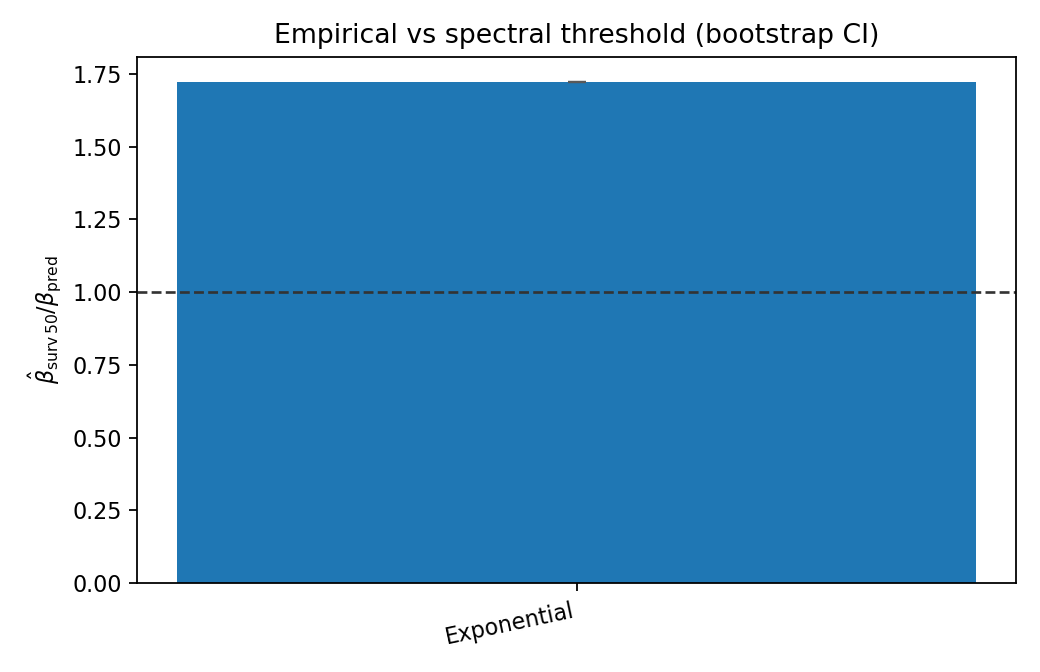
\includegraphics[width=0.62\linewidth]{fig_er_threshold_ratio_bar.png}
  \caption{Ratio $\hat{\beta}_{\mathrm{surv}\,50}/\beta_{\mathrm{pred}}$ on ER with bootstrap error bars (when non-degenerate); dashed line at $1$ (spectral benchmark $c{=}1$). Exponential and lognormal hit the $\beta$ grid ceiling.}
  \label{fig:ratio-bar}
\end{figure}

\begin{figure}[htbp]
  \centering
  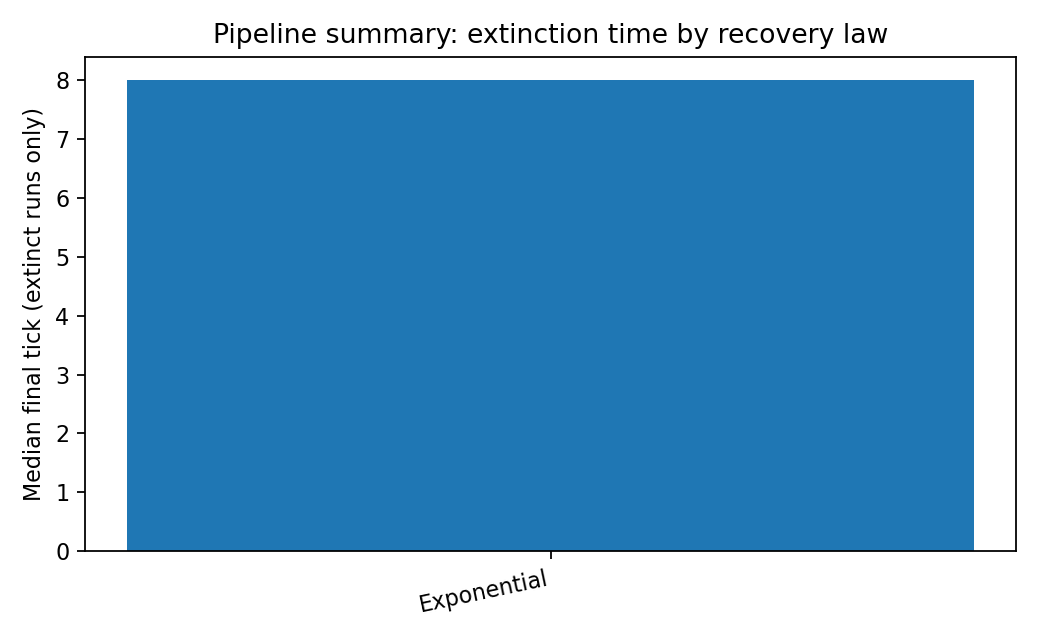
\includegraphics[width=0.62\linewidth]{fig_er_median_extinct_tick.png}
  \caption{Median \texttt{bs-out-final-tick} among extinct runs (pipeline summary per recovery regime on ER). Power-law recovery yields substantially longer extinction times than exponential or lognormal in this summary.}
  \label{fig:extinct-med}
\end{figure}

\subsection{Microscopic vs.\ mean-field prevalence}
Experiment \texttt{08-dynamics-trajectory-ER} records per-tick microscopic prevalence (grp-SIS) and the homogeneous mean-field SIS prevalence updated in the same model. Figure~\ref{fig:traj} shows a single replicate: the two trajectories track closely, while stochastic extinction can end the microscopic run early (exit when no infected remain).

\begin{figure}[htbp]
  \centering
  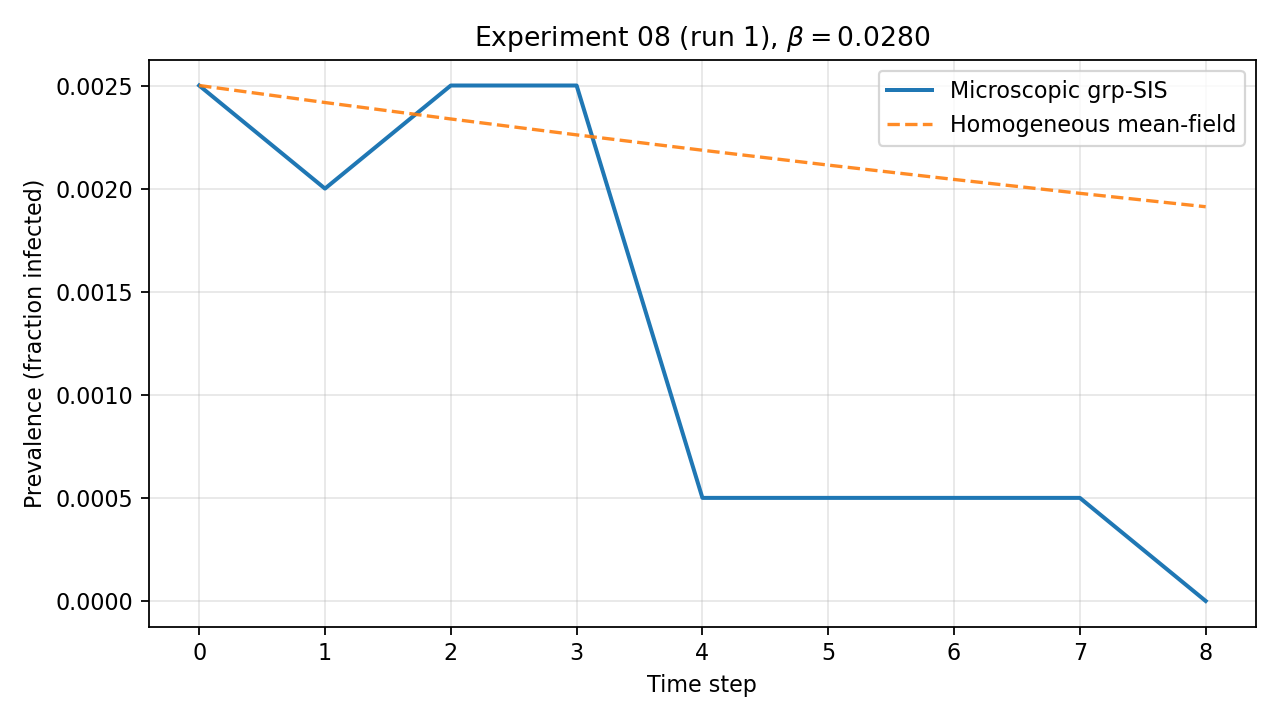
\includegraphics[width=0.82\linewidth]{fig_er_prevalence_trajectory.png}
  \caption{One BehaviorSpace run from \texttt{08-dynamics-trajectory-ER}: microscopic prevalence vs.\ NetLogo mean-field SIS curve at the same parameters.}
  \label{fig:traj}
\end{figure}

\section{Discussion}

\paragraph{Spectral benchmark vs.\ ABM survival (RQ1).}
The empirical $\hat{\beta}_{\mathrm{surv}\,50}$ lies clearly above $\beta_{\mathrm{pred}}$: in $\tau$-space, $\hat{\tau}_{50}=\hat{\beta}_{\mathrm{surv}\,50}\mathbb{E}[W]$ corresponds to an effective multiplier $c\approx \hat{\tau}_{50}\,\lambda_{\max}$ of about $1.58$--$1.72$ on our grid, not $c{=}1$. So the mean-field spectral line is best read as a \emph{scale} or optimistic bound, not a sharp critical value, for this discrete-time, finite-$N$, agent-based grp-SIS implementation. Finite-size effects, discretisation, and spatial correlations beyond mean field are the usual explanations; the trajectory check (Figure~\ref{fig:traj}) shows that the \emph{homogeneous} mean-field equation itself matches the simulation when both are defined on the same state variables, so the gap in Table~\ref{tab:thresholds} is about \emph{where survival becomes likely} in the stochastic model, not about a coding inconsistency between ODE and micro-dynamics.

\paragraph{Recovery shape (RQ2) and dynamics (RQ3).}
The original hypothesis emphasised easier persistence under heavy tails at fixed $\mathbb{E}[W]$. On this ER instance and $\beta$ grid, we do not see a uniform lowering of $\hat{\beta}_{\mathrm{surv}\,50}$ for \emph{both} heavy-tailed regimes: lognormal matches exponential at the grid cap, while power-law recovery crosses $50\%$ at a slightly lower $\beta$. Thus RQ2 receives a nuanced answer---possible ordering effects between specific heavy-tailed laws rather than a single ``heavy tail'' shift. For RQ3, the median extinction-time summary (Figure~\ref{fig:extinct-med}) supports the view that recovery shape reshapes \emph{transient} and extinction behaviour more visibly than a shared spectral $\beta_{\mathrm{pred}}$ might suggest: Tang power-law recovery is associated with longer extinction times in the pipeline summary. A fuller answer would examine extinction-time \emph{distributions} by $\beta$ (not only the aggregated median) and persistence of late-window prevalence.

\paragraph{Limitations.}
Estimators that hit the largest $\beta$ are censored: extending the $\beta$ grid (or fitting a logistic dose--response) would sharpen $\hat{\beta}_{\mathrm{surv}\,50}$ for exponential and lognormal curves (see the estimation-protocol improvement mark in Methods). We use one large ER draw per seed; repeating over graph realisations would separate topological from process noise. Experiments \texttt{02}--\texttt{04} in the XML add other interconnection structures; the present report focuses on the ER baseline aligned with $\lambda_{\max}$ from \path{output/edges/edges_ER_10001.csv}. The study concerns synthetic disease transmission only; no human or animal data are involved.

\peerreviewmark{RQ3 would be strengthened by extinction-time \emph{distributions} conditional on $\beta$ (not only regime-level medians), as the proposal anticipated. The present figures summarise one aggregate per recovery law; a heatmap or faceted survival curves by $\beta$ would better separate threshold shifts from transient variability.}

\section{Conclusion}
\label{sec:conclusion}

For grp-SIS on a moderately dense ER graph with fixed mean recovery time, the spectral benchmark $\beta_{\mathrm{pred}}=1/(\lambda_{\max}\mathbb{E}[W])$ remains a useful scale but systematically underestimates the $\beta$ at which survival at the fixed horizon becomes common in this ABM: in $\tau$-space, $\hat{\tau}_{50}/\tau_{\mathrm{pred}}$ is about $1.58$--$1.72$ on our grid, not $c{=}1$. A standard heterogeneous mean-field $\beta$ from degree moments moves only slightly relative to $\beta_{\mathrm{pred}}$ and does not absorb that gap. Differences between recovery \emph{laws} show up in threshold ordering at finite resolution (power law vs.\ exponential/lognormal on this sweep) and more clearly in extinction-time summaries. Overall, heavy-tailed recovery does not uniformly lower the empirical survival threshold relative to Markovian recovery here; it interacts with the chosen law and with censoring. Extending $\beta$ sweeps, adding graph ensembles, and analysing extinction-time distributions conditional on $\beta$ would further connect Tang-style non-Markovian recovery to spectral threshold practice.

\section*{Data and code availability}
\phantomsection
\addcontentsline{toc}{section}{Data and code availability}

BehaviorSpace table exports, edge lists, and aggregated threshold CSVs are under \path{output/} in the project repository. The NetLogo model and experiment definitions are in \path{netlogo/virus_simulation.nlogox} and \path{netlogo/behaviorspace_experiments.xml}. Figures in this PDF were generated with \path{scripts/export_report_figures.py}.

\begin{thebibliography}{99}

\bibitem{ErdosRenyi1959}
P.~Erd\H{o}s and A.~R\'enyi.
\newblock On random graphs.
\newblock \emph{Publ.\ Math.\ Debrecen} \textbf{6}, 290--297 (1959).

\bibitem{Cator2013}
E.~Cator, R.~van de Bovenkamp, and P.~Van Mieghem.
\newblock Susceptible--infected--susceptible epidemics on networks with general infection and cure times.
\newblock \emph{Phys.\ Rev.\ E} \textbf{87}, 062816 (2013).

\bibitem{Chakrabarti2008}
D.~Chakrabarti, Y.~Wang, C.~Wang, J.~Leskovec, and C.~Faloutsos.
\newblock Epidemic thresholds in real networks.
\newblock \emph{ACM Trans.\ Inf.\ Syst.\ Secur.} \textbf{10}, 13 (2008).


\bibitem{PastorSatorras2015}
R.~Pastor-Satorras, C.~Castellano, P.~Van Mieghem, and A.~Vespignani.
\newblock Epidemic processes in complex networks.
\newblock \emph{Rev.\ Mod.\ Phys.} \textbf{87}, 925--979 (2015).


\bibitem{Tang2025}
J.~Tang, Y.~Yao, M.~Xie, and M.~Feng.
\newblock SIS epidemic modelling on homogeneous networked system: General recovering process and mean-field perspective.
\newblock \emph{Appl.\ Math.\ Modelling} (2025); preprint arXiv:2505.12290v2.

\bibitem{VanMieghem2011}
P.~Van Mieghem.
\newblock The $N$-intertwined SIS epidemic network model.
\newblock \emph{Computing} \textbf{93}, 147--169 (2011).

\end{thebibliography}

\clearpage
\appendix
\section{BehaviorSpace experiment configurations (NetLogo)}
\label{app:behaviorspace}

This appendix documents the NetLogo BehaviorSpace experiments used in this project as defined in \path{netlogo/behaviorspace_experiments.xml} (and mirrored into \path{netlogo/virus_simulation.nlogox} for headless execution). It lists the experiment names, repetitions, stopping rules, reported metrics, and parameter sweeps so that results can be reproduced without opening the NetLogo GUI.

% Prevent overfull boxes due to long monospace parameter names/strings.
\sloppy

\subsection{Common elements}
\begin{itemize}[leftmargin=*]
  \item \textbf{Model}: \path{netlogo/virus_simulation.nlogox} (NetLogo 7.x).
  \item \textbf{Exit condition (threshold experiments)}: runs stop at the time horizon or absorption,
  \[
    (\texttt{ticks} \ge \texttt{sim-tick-limit}) \ \ \text{or}\ \ (\text{no infected agents}).
  \]
  \item \textbf{Key controlled settings (reported below)}: network specification (\texttt{interconnection-structure}, \texttt{network-type}, \texttt{expt-seed}, \texttt{num-nodes}, \texttt{avg-degree}), epidemic parameters (\texttt{infection-prob}, \texttt{recovery-mean}, recovery distribution chooser and its parameters), initial condition (\texttt{initial-infected}), and horizon (\texttt{max-ticks}).
\end{itemize}

\subsection{Experiment 01: network export}
\paragraph{\texttt{01-export-networks}}
\begin{itemize}[leftmargin=*]
  \item \textbf{Purpose}: export edge lists for subsequent computation of $\lambda_{\max}$ and mean-field reference quantities.
  \item \textbf{Repetitions}: 1.
  \item \textbf{Setup (summary)}: disables collection of epidemic metrics; calls \texttt{export-network-edges} to write \path{output/edges/edges_\{net\}\_\{seed\}.csv}.
  \item \textbf{Exit condition}: \texttt{true} (immediate after export).
  \item \textbf{Metrics}: \texttt{safe-net-label}, \texttt{count links}, \texttt{num-nodes}, \texttt{bs-out-mean-degree}.
  \item \textbf{Constants and sweeps}:
  \begin{itemize}[leftmargin=*]
    \item \texttt{interconnection-structure} $\in$ \{\texttt{"Lattice4"}, \texttt{"Ring"}, \texttt{"other"}\}.
    \item \texttt{network-type} $=$ \texttt{"Erdos-Renyi (random)"} (used when \texttt{interconnection-structure="other"}).
    \item \texttt{expt-seed} $=$ 10001.
    \item \texttt{num-nodes} $\in$ \{200, 2000\}.
    \item \texttt{avg-degree} $=$ 6; \texttt{rewiring-prob} $=$ 0.07; \texttt{initial-infected} $=$ 5; \texttt{max-ticks} $=$ 3000.
  \end{itemize}
\end{itemize}

\subsection{Experiments 02--04: coarse threshold sweeps on regular structures}
\paragraph{\texttt{02-threshold-exponential}}
\begin{itemize}[leftmargin=*]
  \item \textbf{Repetitions}: 8.
  \item \textbf{Recovery law}: \texttt{"exponential"}.
  \item \textbf{Metrics}: \texttt{bs-out-extinct}, \texttt{bs-out-final-tick}, \texttt{bs-out-late-mean-prevalence}, \texttt{bs-out-tau-sim}, \texttt{bs-out-mean-degree}.
  \item \textbf{Constants and sweeps}: \texttt{interconnection-structure} $\in$ \{\texttt{"Lattice4"}, \texttt{"Ring"}\}; \texttt{expt-seed}$=$1001; \texttt{num-nodes}$=$200; \texttt{avg-degree}$=$6; \texttt{initial-infected}$=$5; \texttt{recovery-mean}$=$5; \texttt{max-ticks}$=$3000; stepped \texttt{infection-prob} from 0.02 to 0.56 in steps of 0.03.
\end{itemize}

\paragraph{\texttt{03-threshold-power-law-Tang}}
\begin{itemize}[leftmargin=*]
  \item \textbf{Repetitions}: 8.
  \item \textbf{Recovery law}: \texttt{"power law (Tang)"} with \texttt{power-law-lambda}$=$4.24.
  \item \textbf{Metrics}: same as experiment~02.
  \item \textbf{Constants and sweeps}: same as experiment~02, with the additional constant \texttt{power-law-lambda}$=$4.24.
\end{itemize}

\paragraph{\texttt{04-threshold-lognormal-Tang}}
\begin{itemize}[leftmargin=*]
  \item \textbf{Repetitions}: 8.
  \item \textbf{Recovery law}: \texttt{"lognormal (Tang)"} with \texttt{lognormal-sigma}$=$1.
  \item \textbf{Metrics}: same as experiment~02.
  \item \textbf{Constants and sweeps}: same as experiment~02, with the additional constant \texttt{lognormal-sigma}$=$1.
\end{itemize}

\subsection{Experiments 05--07: ER baseline experiments (main results)}
\paragraph{\texttt{05-baseline-empirical-threshold-ER}}
\begin{itemize}[leftmargin=*]
  \item \textbf{Repetitions}: 24.
  \item \textbf{Network}: \texttt{interconnection-structure="other"}, \texttt{network-type="Erdos-Renyi (random)"}; fixed \texttt{expt-seed}$=$10001; \texttt{num-nodes}$=$2000; \texttt{avg-degree}$=$6.
  \item \textbf{Recovery law}: \texttt{"exponential"} with \texttt{recovery-mean}$=$5.
  \item \textbf{Horizon}: \texttt{max-ticks}$=$10000.
  \item \textbf{Metrics}: \texttt{bs-out-extinct}, \texttt{bs-out-final-tick}, \texttt{bs-out-late-mean-prevalence}, \texttt{bs-out-tau-sim}, \texttt{bs-out-mean-degree}.
  \item \textbf{Sweep}: stepped \texttt{infection-prob} from 0.018 to 0.048 in steps of 0.002.
\end{itemize}

\paragraph{\texttt{06-baseline-ER-power-law-Tang}}
\begin{itemize}[leftmargin=*]
  \item \textbf{Repetitions}: 24 (same ER network instance as experiment~05; process noise via repetitions).
  \item \textbf{Recovery law}: \texttt{"power law (Tang)"} with \texttt{recovery-mean}$=$5 and \texttt{power-law-lambda}$=$4.24.
  \item \textbf{Horizon, metrics, sweep}: identical to experiment~05.
\end{itemize}

\paragraph{\texttt{07-baseline-ER-lognormal-Tang}}
\begin{itemize}[leftmargin=*]
  \item \textbf{Repetitions}: 24 (same ER network instance as experiment~05; process noise via repetitions).
  \item \textbf{Recovery law}: \texttt{"lognormal (Tang)"} with \texttt{recovery-mean}$=$5 and \texttt{lognormal-sigma}$=$1.
  \item \textbf{Horizon, metrics, sweep}: identical to experiment~05.
\end{itemize}

\subsection{Experiment 08: prevalence trajectories (grp-SIS vs mean-field)}
\paragraph{\texttt{08-dynamics-trajectory-ER}}
\begin{itemize}[leftmargin=*]
  \item \textbf{Purpose}: export per-tick prevalence for the microscopic grp-SIS simulation and the in-model homogeneous mean-field SIS curve for the same parameters.
  \item \textbf{Repetitions}: 5.
  \item \textbf{RunMetricsEveryStep}: \texttt{true} (per-tick table export).
  \item \textbf{Network and initial condition}: ER baseline with \texttt{expt-seed}$=$10001; \texttt{num-nodes}$=$2000; \texttt{avg-degree}$=$6; \texttt{initial-infected}$=$5.
  \item \textbf{Recovery law}: \texttt{"exponential"} with \texttt{recovery-mean}$=$5.
  \item \textbf{Horizon}: \texttt{max-ticks}$=$2000.
  \item \textbf{Infection strength}: \texttt{infection-prob}$=$0.028 (single value).
  \item \textbf{Metrics}: \texttt{bs-out-prev-grp}, \texttt{bs-out-prev-mf}, \texttt{bs-out-count-S}, \texttt{bs-out-count-I}, \texttt{bs-out-mean-degree}.
\end{itemize}

\end{document}
